\subsection{20 августа. пер. Уллукёль Восточный (1А*)}
\textit{Метеоусловия: утром, днём ясно, вечером~--- переменная облачность, тепло.}

%\begin{minipage}{0.9\linewidth}
\begin{table}[h!]
	\begin{tabular}{|c|c|c|c|c|c|} 
		\hline 
		Этап & Время начала & Время окончания & ЧХВ & Пройдено по горизонтали, км & Набор / сброс, м \\ 	
		\hline 
		От м/н до начала курумника & & & & \\ 
		От курумника до начала морен &&&& \\ 
		По моренам до камня-моста &&&& \\ 
		До кулуара &&&& \\
		По осыпи под скалы &&&&\\ 
		Вдоль скал до начала снежника &&&&
		\end{tabular}
	\end{table}
%\end{minipage}

\begin{figure}[h!]
	\centering
	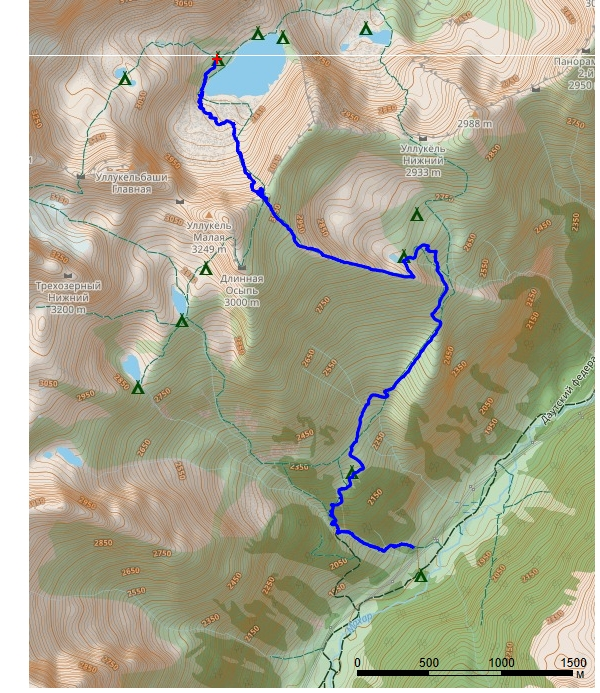
\includegraphics[angle=0, width=0.7\linewidth]{../pics/mini_maps/20}
	\label{fig:mini_20}
\end{figure}

Подъём дежурных в 04:30, общий подъём в 05:00. Выход группы в 07:30 (рис.~\ref{fig:20aug1.jpg}).

\begin{figure}[h!]
	\centering
	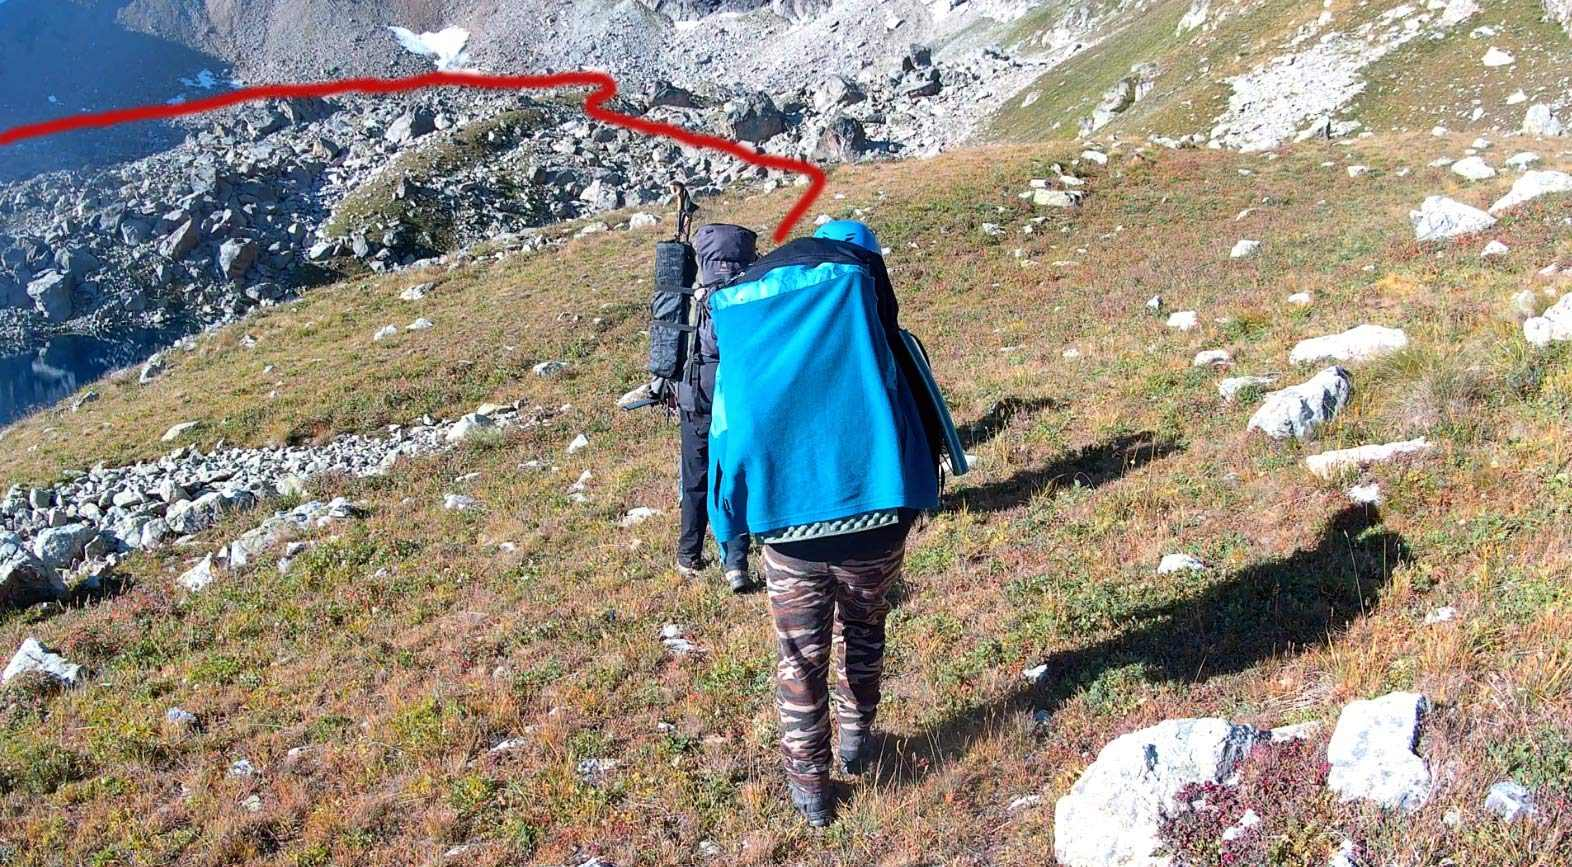
\includegraphics[width=0.7\linewidth]{../pics/20aug1.jpg}
	\caption{Подход под перевал от м.н.}
	\label{fig:20aug1.jpg}
\end{figure}


 Движемся по разведанному вчера маршруту по крупной осыпи в обход южной оконечности озера. На одном из привалов участнице (Наташе Мироновой) становится нехорошо, и часть пути (ок. 15 мин. ЧХВ) она проходит без рюкзака. Пока доносим рюкзак, группа фотографируется на фоне озера на небольшом зелёном гребешке (рис.~\ref{fig:DSC_0907}).
 
 \begin{figure}[h!]
 	\centering
 	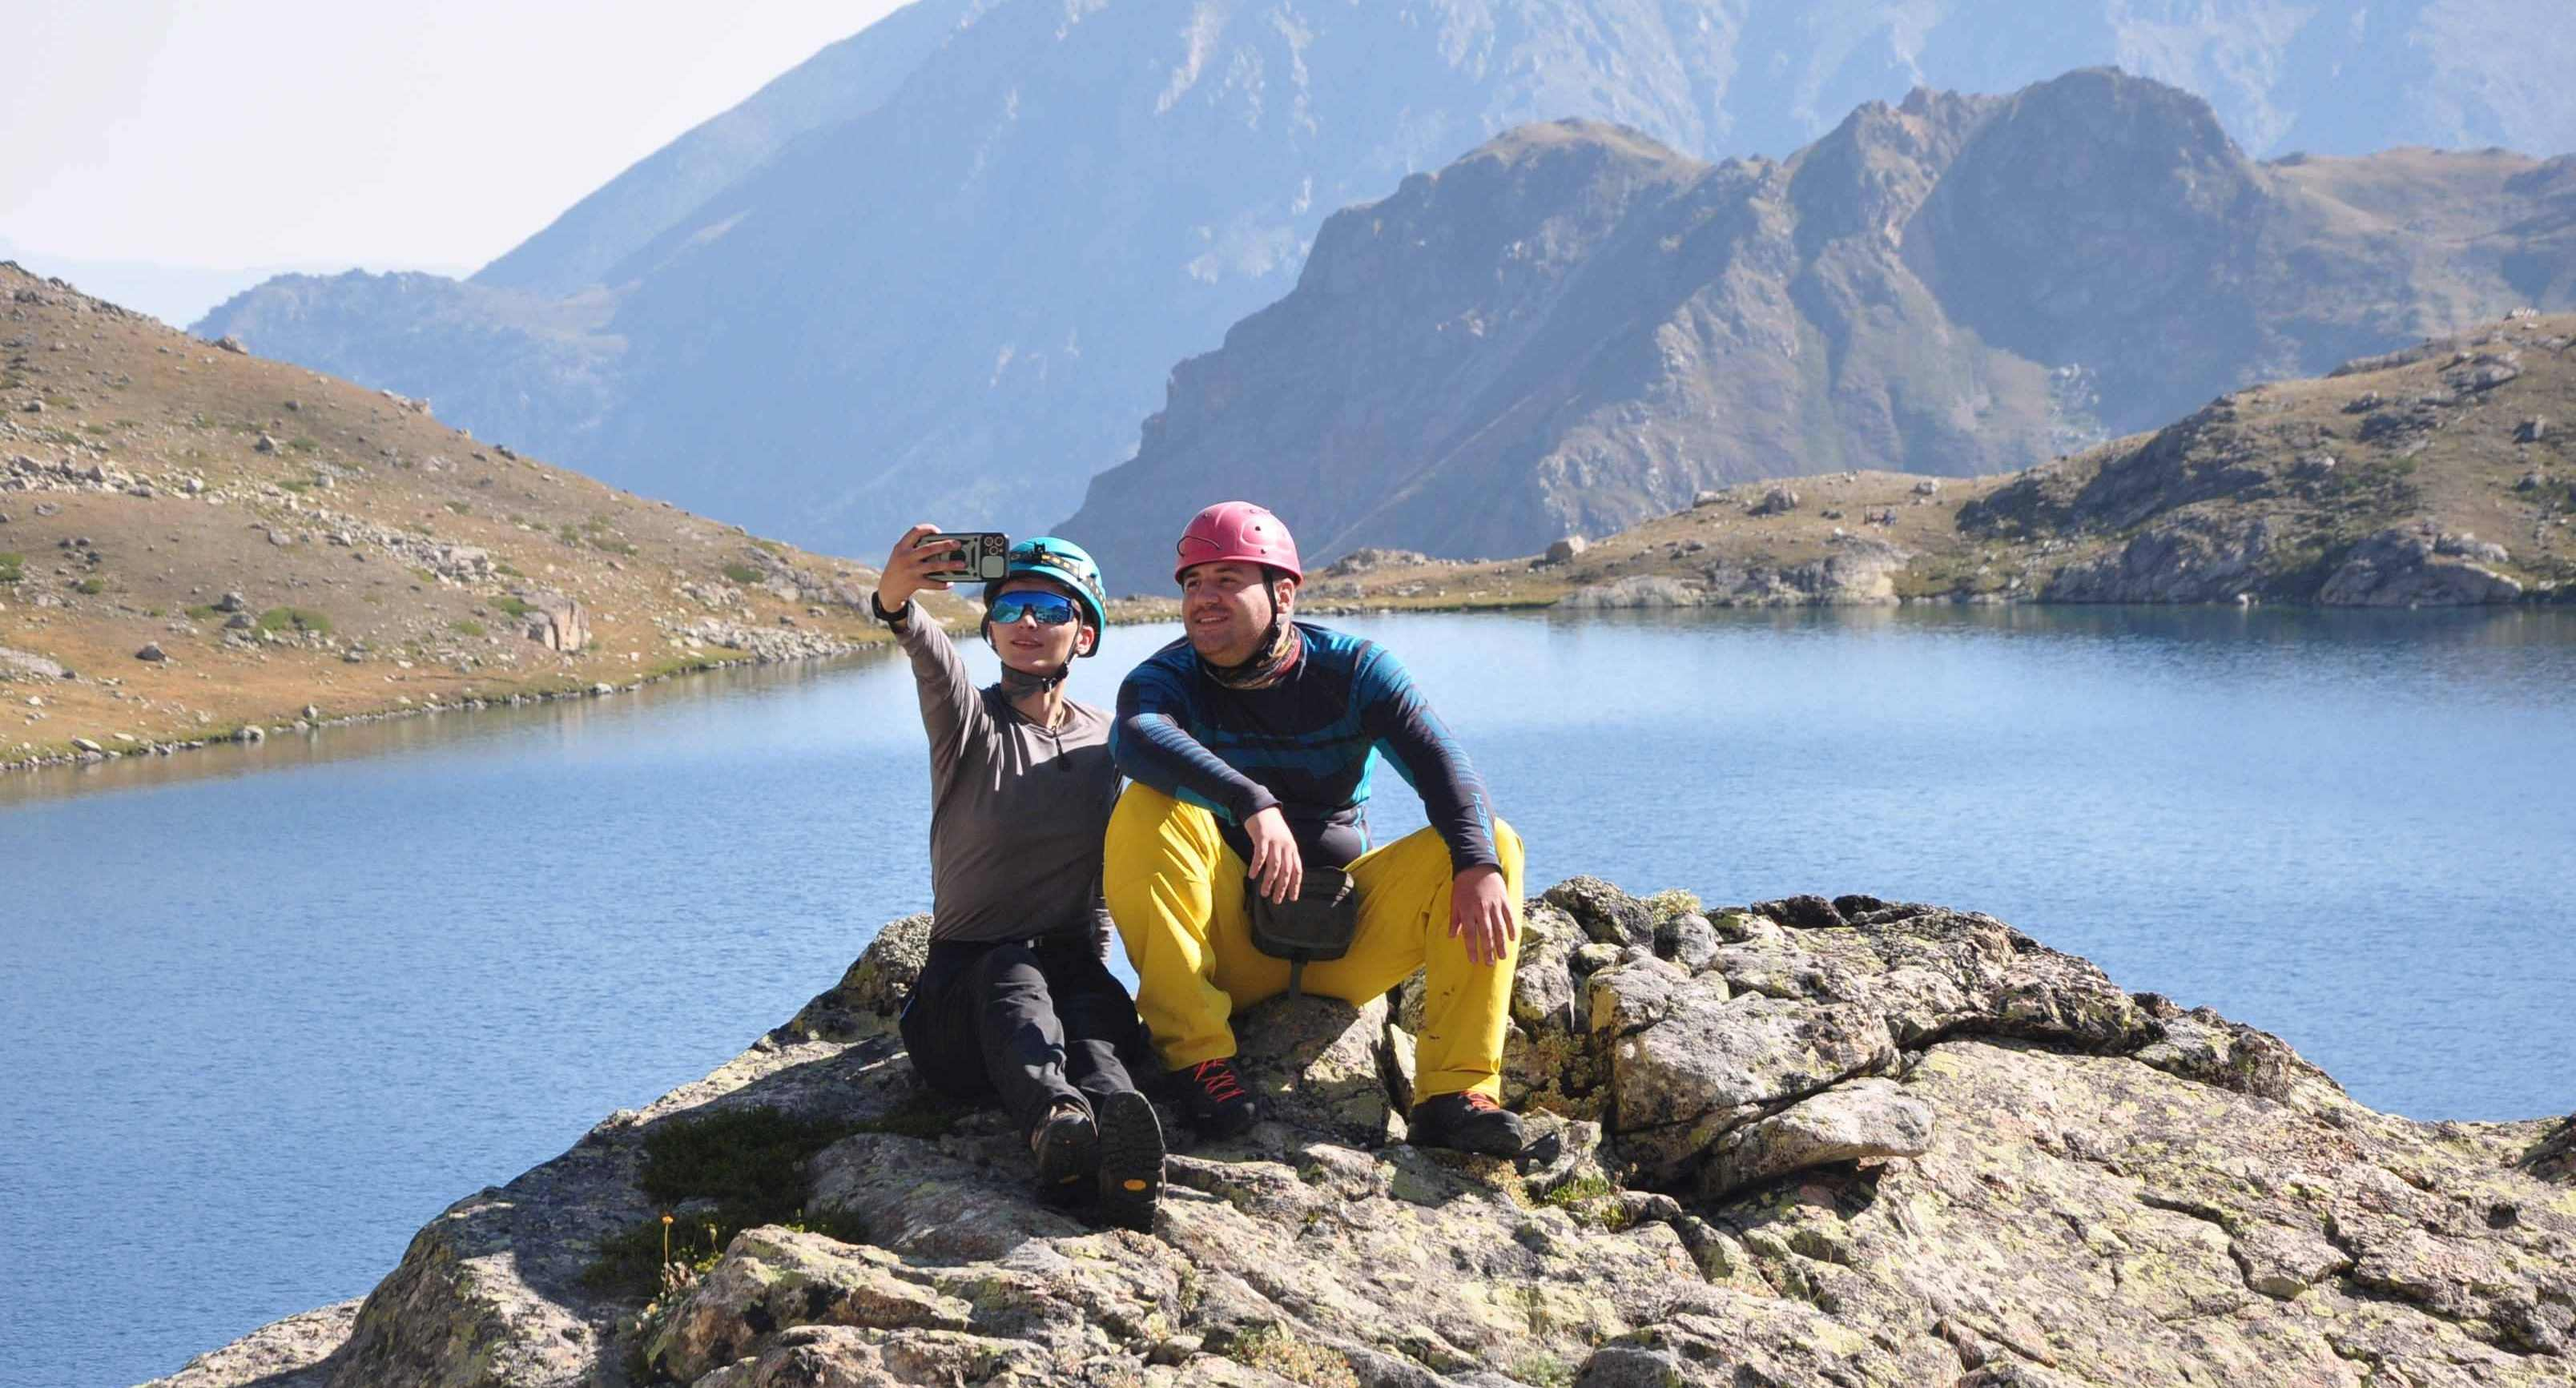
\includegraphics[width=0.7\linewidth]{../pics/DSC_0907}
 	\caption{Фоткаемся на фоне озера}
 	\label{fig:DSC_0907}
 \end{figure}
 

Далее движемся на юго-восток по морене до другого зелёного гребешка, ведущего под перевальный взлёт (рис.~\ref{fig:20aug2.jpg}) и в 9:40 выходим на среднюю осыпь перевального взлёта, прижимаясь к правому пхд борту кулуара. Осыпь живая, требует внимания при движении и контроля неопытных участников.

\begin{figure}[h!]
	\centering
	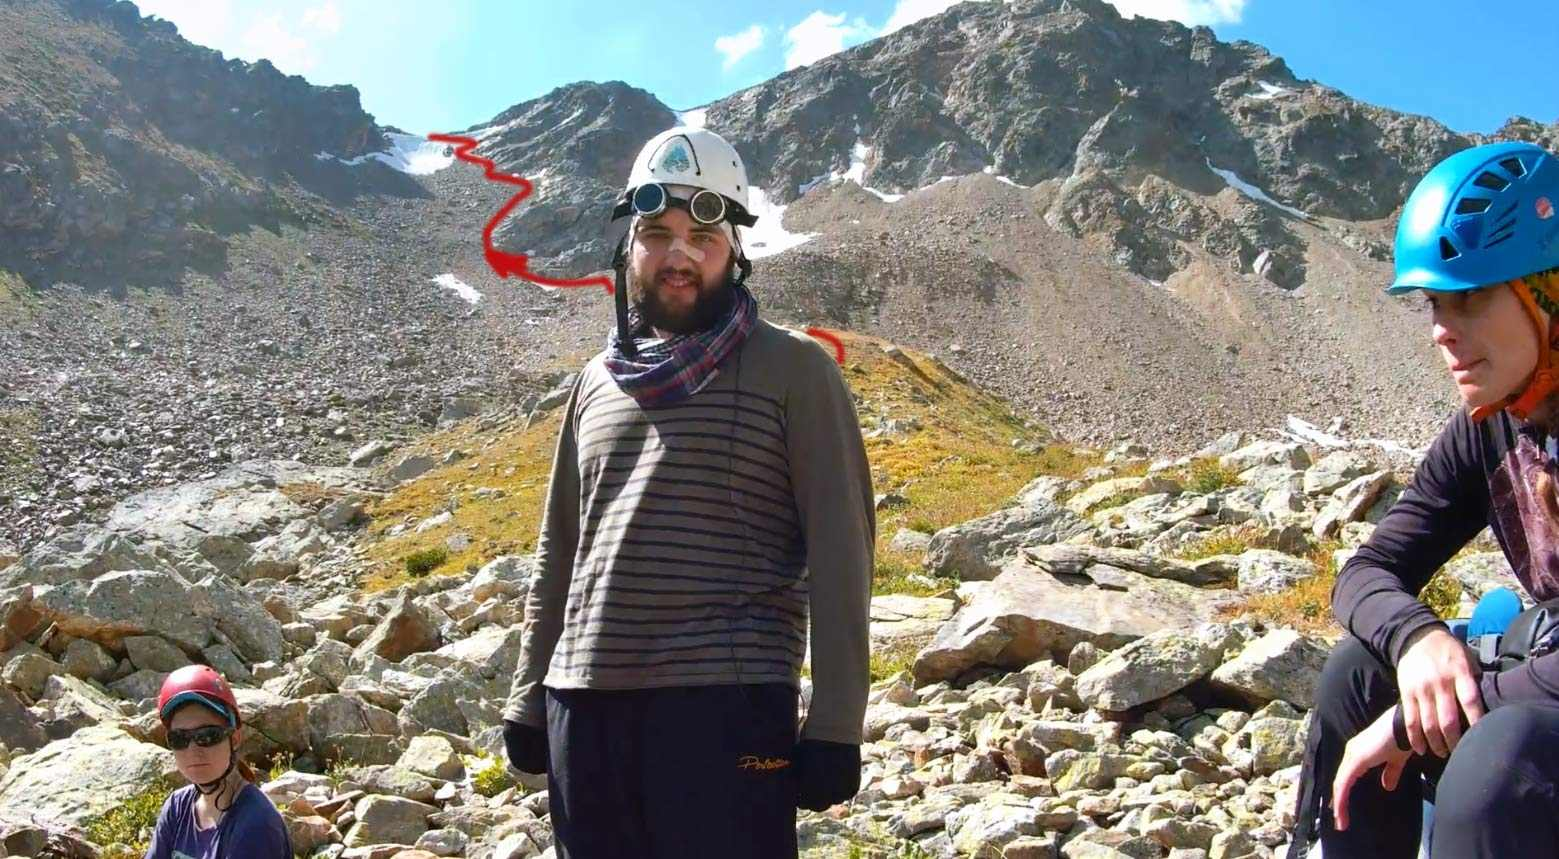
\includegraphics[width=0.7\linewidth]{../pics/20aug2.jpg}
	\caption{Маршрут движения по перевальному взлёту}
	\label{fig:20aug2.jpg}
\end{figure}

Снега на перевальном взлёте почти нет, поэтому руководитель принимает решение двигаться не по линии падения воды, а по правому борту кулуара. Осыпь местами живая, движемся не спеша. В 12:25 достигаем полочки, на уровне которой начинается самая крутая часть перевального взлёта и снежник. Надеваем кошки и движемся косым траверсом влево пхд, чтобы выйти на седловину. Снег мягкий, возможно организовывать ступени, если ставить ногу на всю ступню. На седловине снежного карниза нет, но присутствует удобный снежный карман (рис.~\ref{fig:DSC_0946}). За 70 м тропёжки произвели две смены лидера.

\begin{figure}[h!]
	\centering
	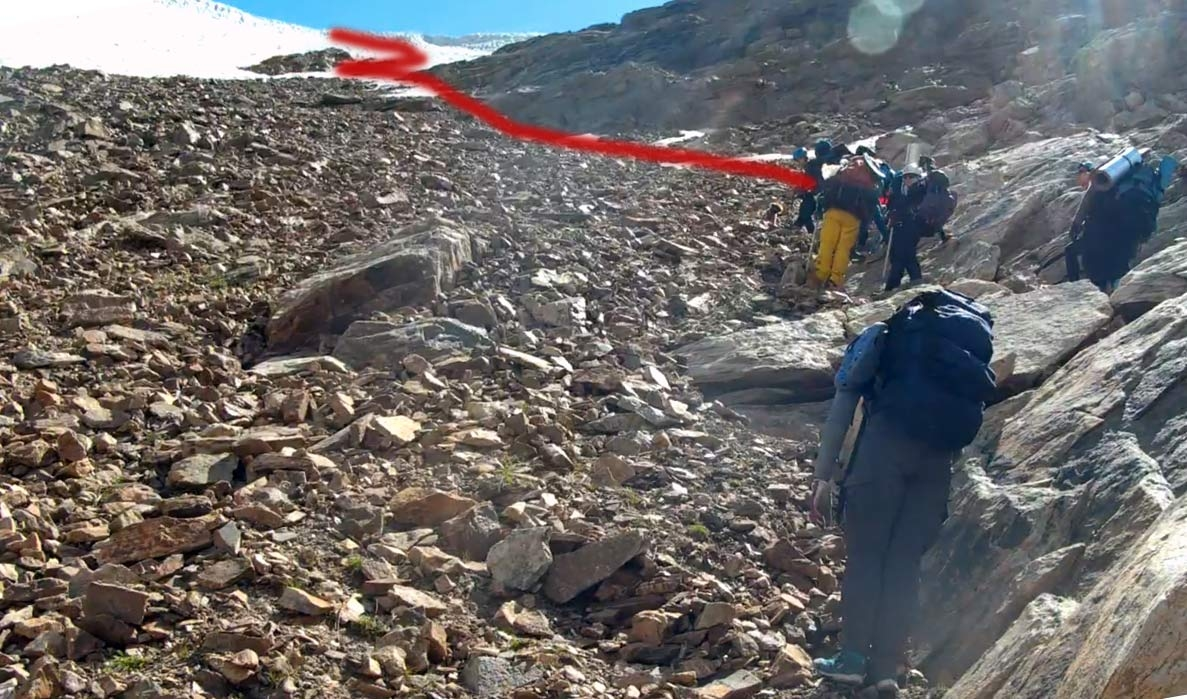
\includegraphics[width=0.7\linewidth]{../pics/20aug3.jpg}
	\caption{Движение по правому пхд борту кулуара}
	\label{fig:20aug3.jpg}
\end{figure}

\begin{figure}[h!]
	\centering
	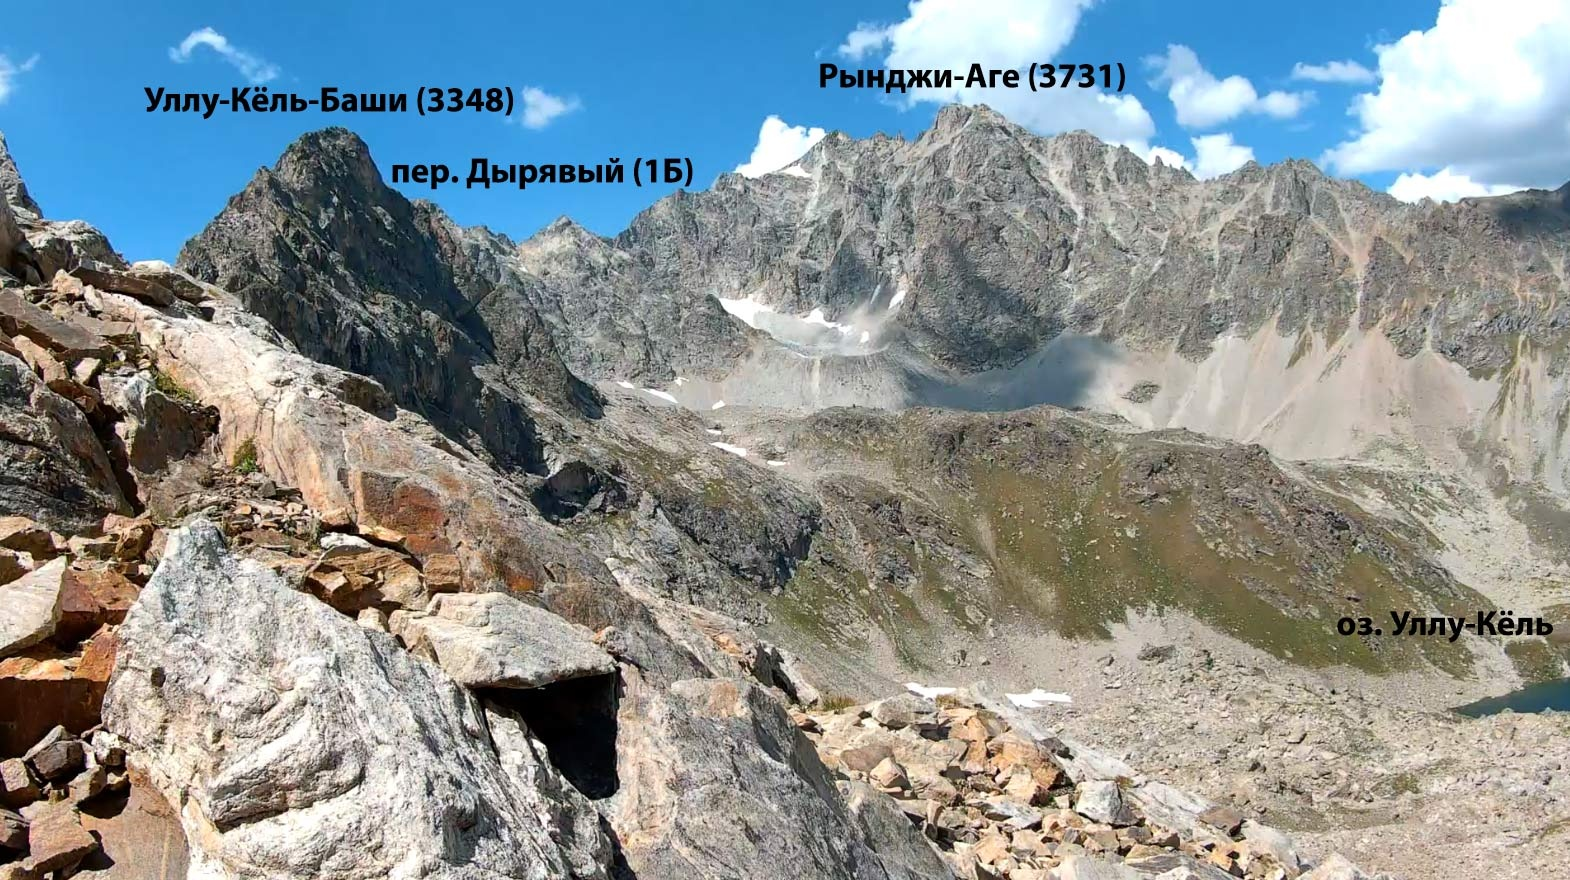
\includegraphics[width=0.7\linewidth]{../pics/20aug4.jpg}
	\caption{Вершины и перевалы цирка Уллу-Кёль}
	\label{fig:20aug4.jpg}
\end{figure}

Когда до снежного кармана (безопасной зоны) оставалось около 3 м по вертикали, лидер, (Катя), срывается. Пролетев 50 метров по снежному склону крутизной 45\degree, Катя не успевает окончательно зарубиться и останавливается только на осыпном склоне, перекувыркнушись через голову. Сразу после падения голосовыми командами убеждаемся, что пострадавшая в сознании. Катя в течение минуты проводит самостоятельный осмотр и убеждается в отсутствии сильных кровотечений. Руководитель и заместитель решают довести группу до безопасной зоны~--- снежного кармана, после чего спуститься к Кате. Последний человек покидает опасную зону спустя 7 минут после срыва, после чего Даша и Лёша спускаются к Кате, убеждаются, что она может идти самостоятельно, дают воду, еду и пуховку. Далее втроём поднимаемся к группе. Катя без рюкзака идёт посередине (рис.~\ref{fig:DSC_0946}).


\begin{figure}[h!]
	\centering
	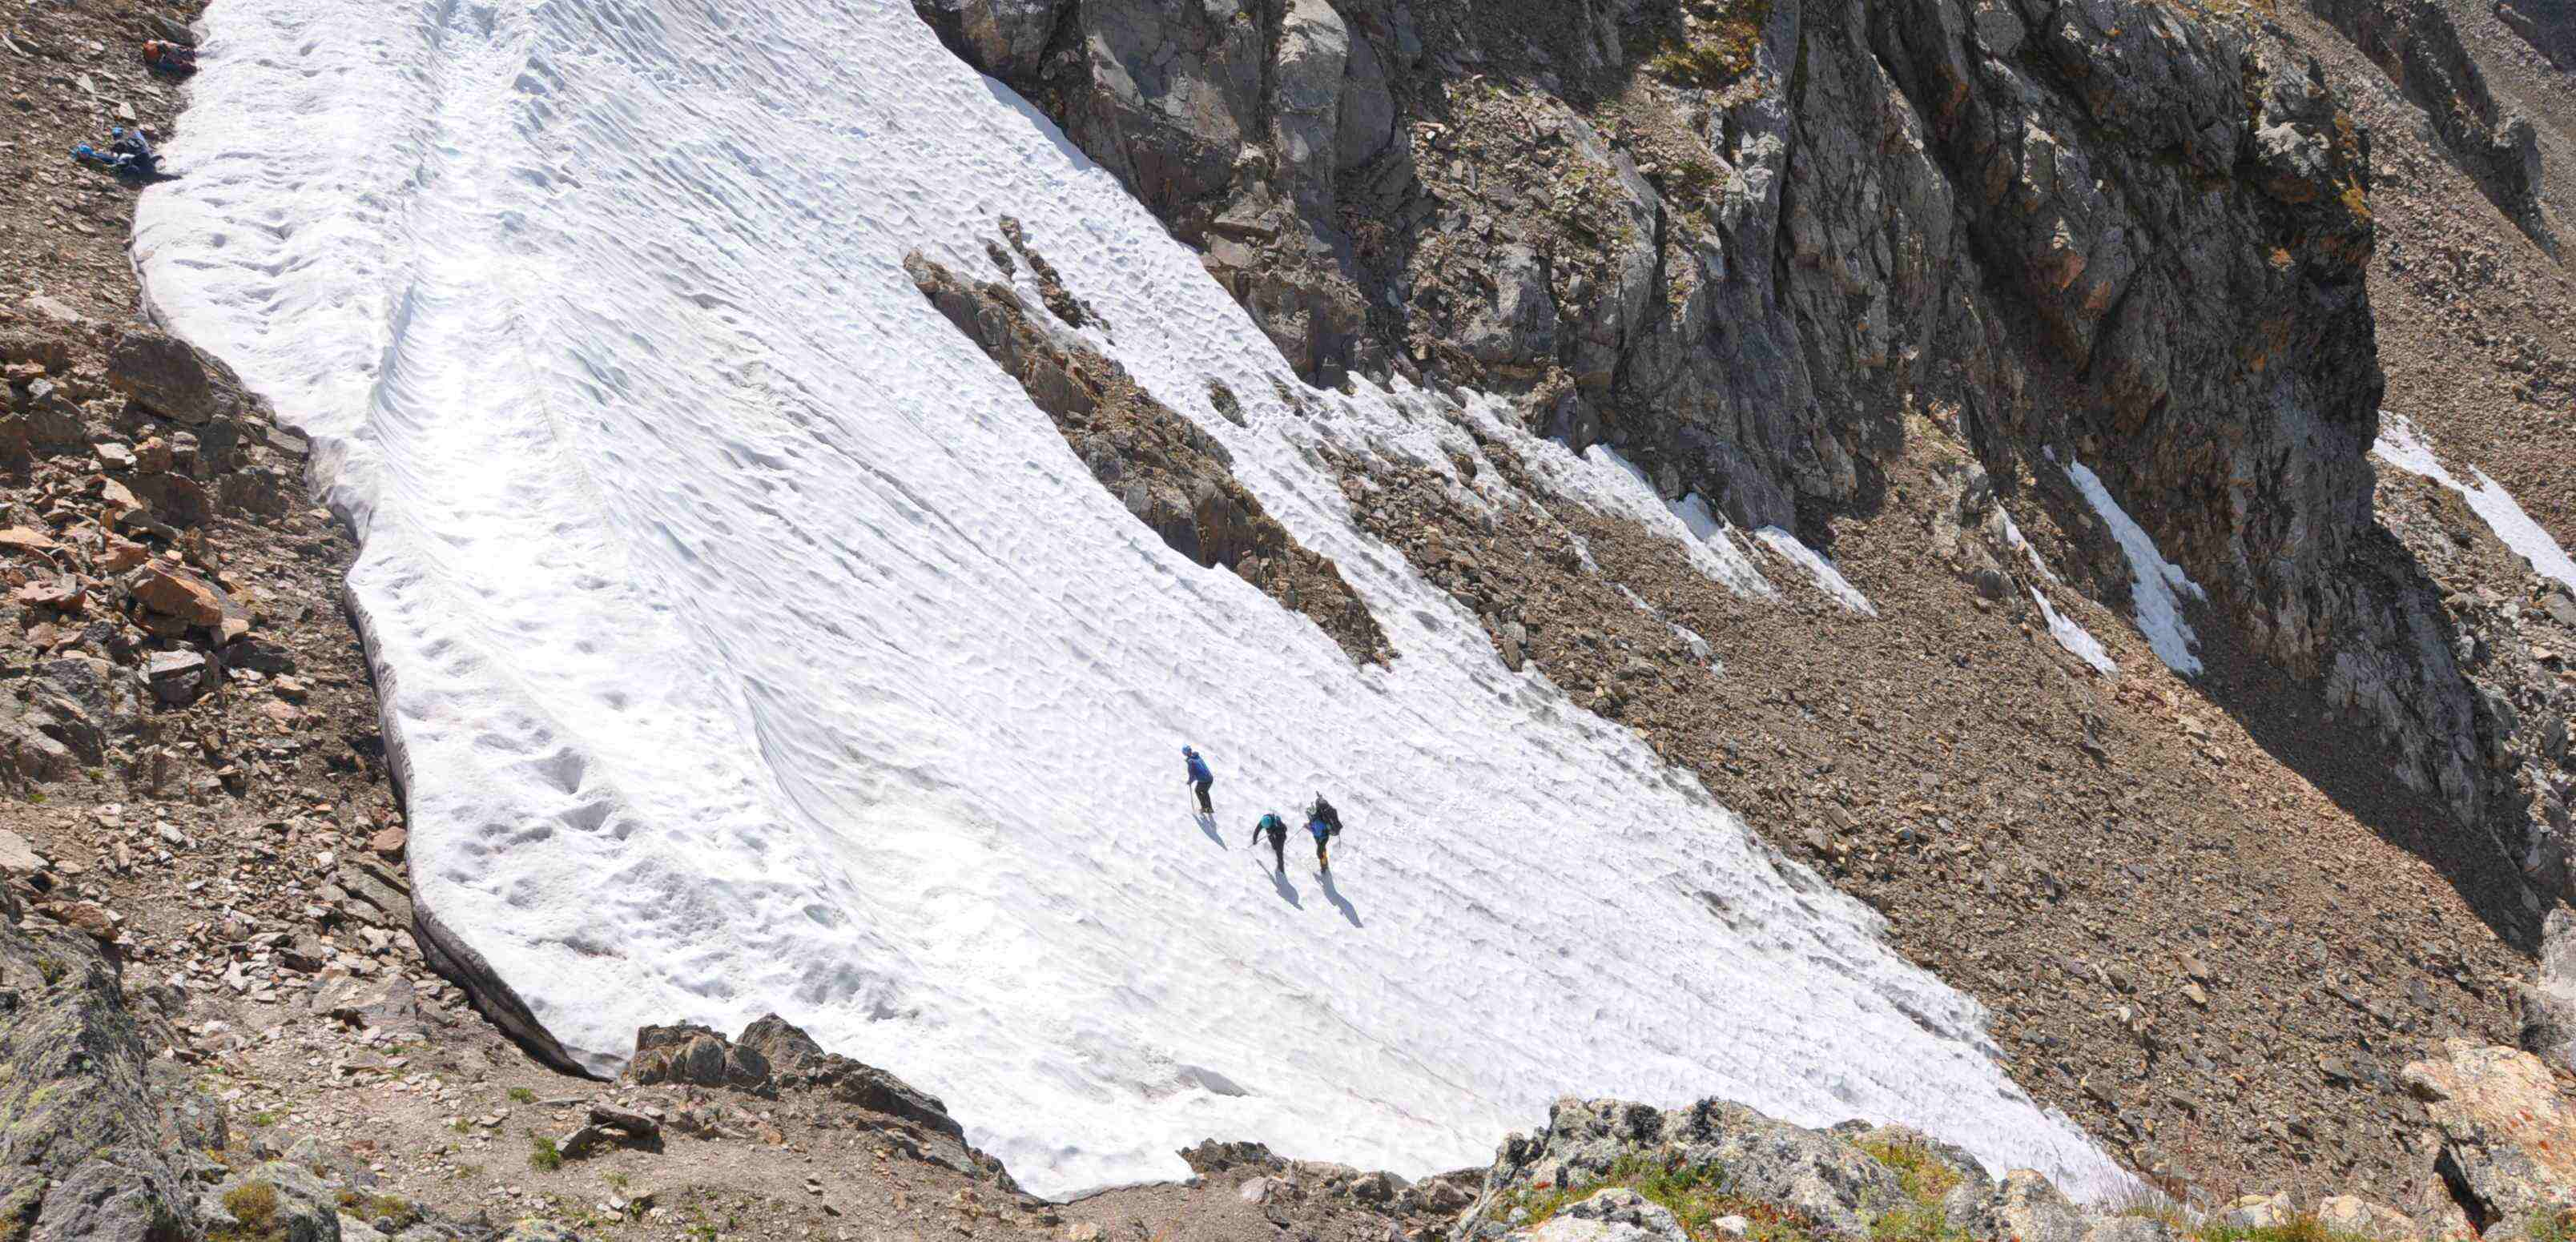
\includegraphics[width=0.7\linewidth]{../pics/DSC_0946.png}
	\caption{Маршрут движения группы по снежнику (красный), траектория срыва участника (синий), маршрут подъёма с сорвавшимся участником (чёрный)}
	\label{fig:DSC_0946}
\end{figure}

Вся группа собирается на седловине в 14:30. Снимаем записку туристов т/к <<Шторм>>, г. Санкт-Петербург, от 09.08.2024.

\begin{figure}[h!]
	\centering
	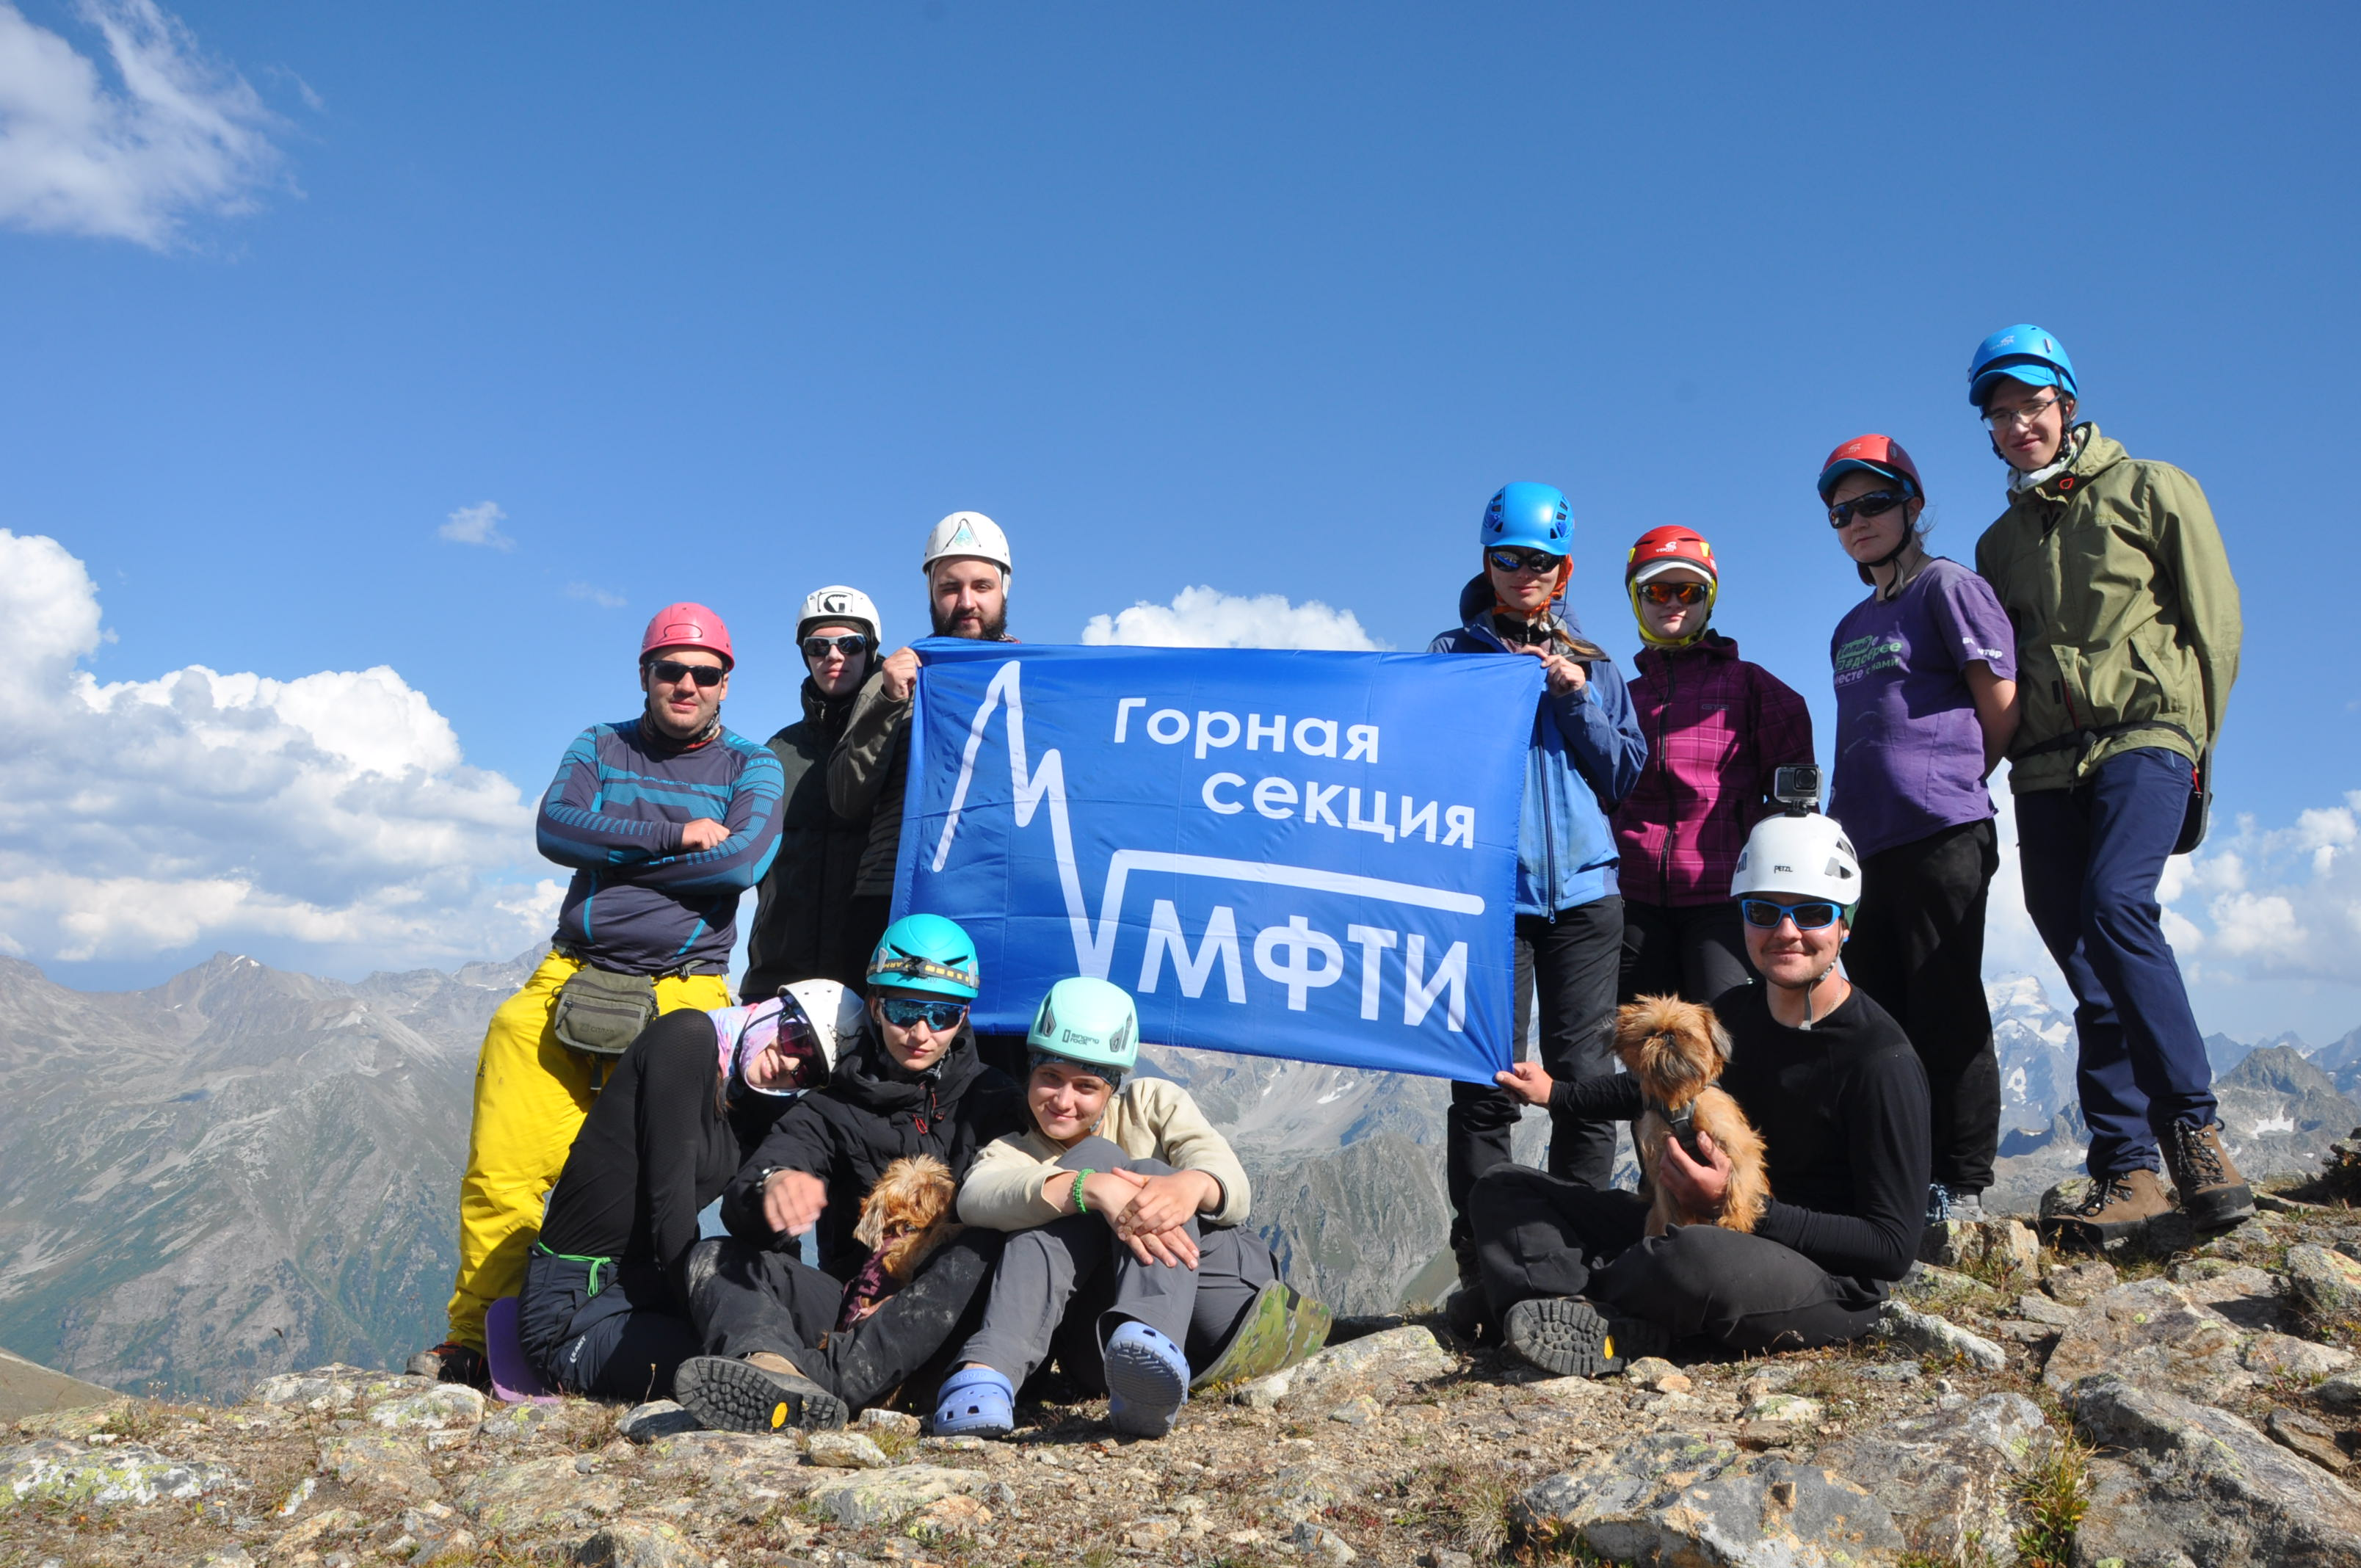
\includegraphics[width=0.7\linewidth]{../pics/DSC_0982}
	\caption{Группа на перевале, вид на д.р. Махар}
	\label{fig:DSC_0982}
\end{figure}

\begin{figure}[h!]
	\centering
	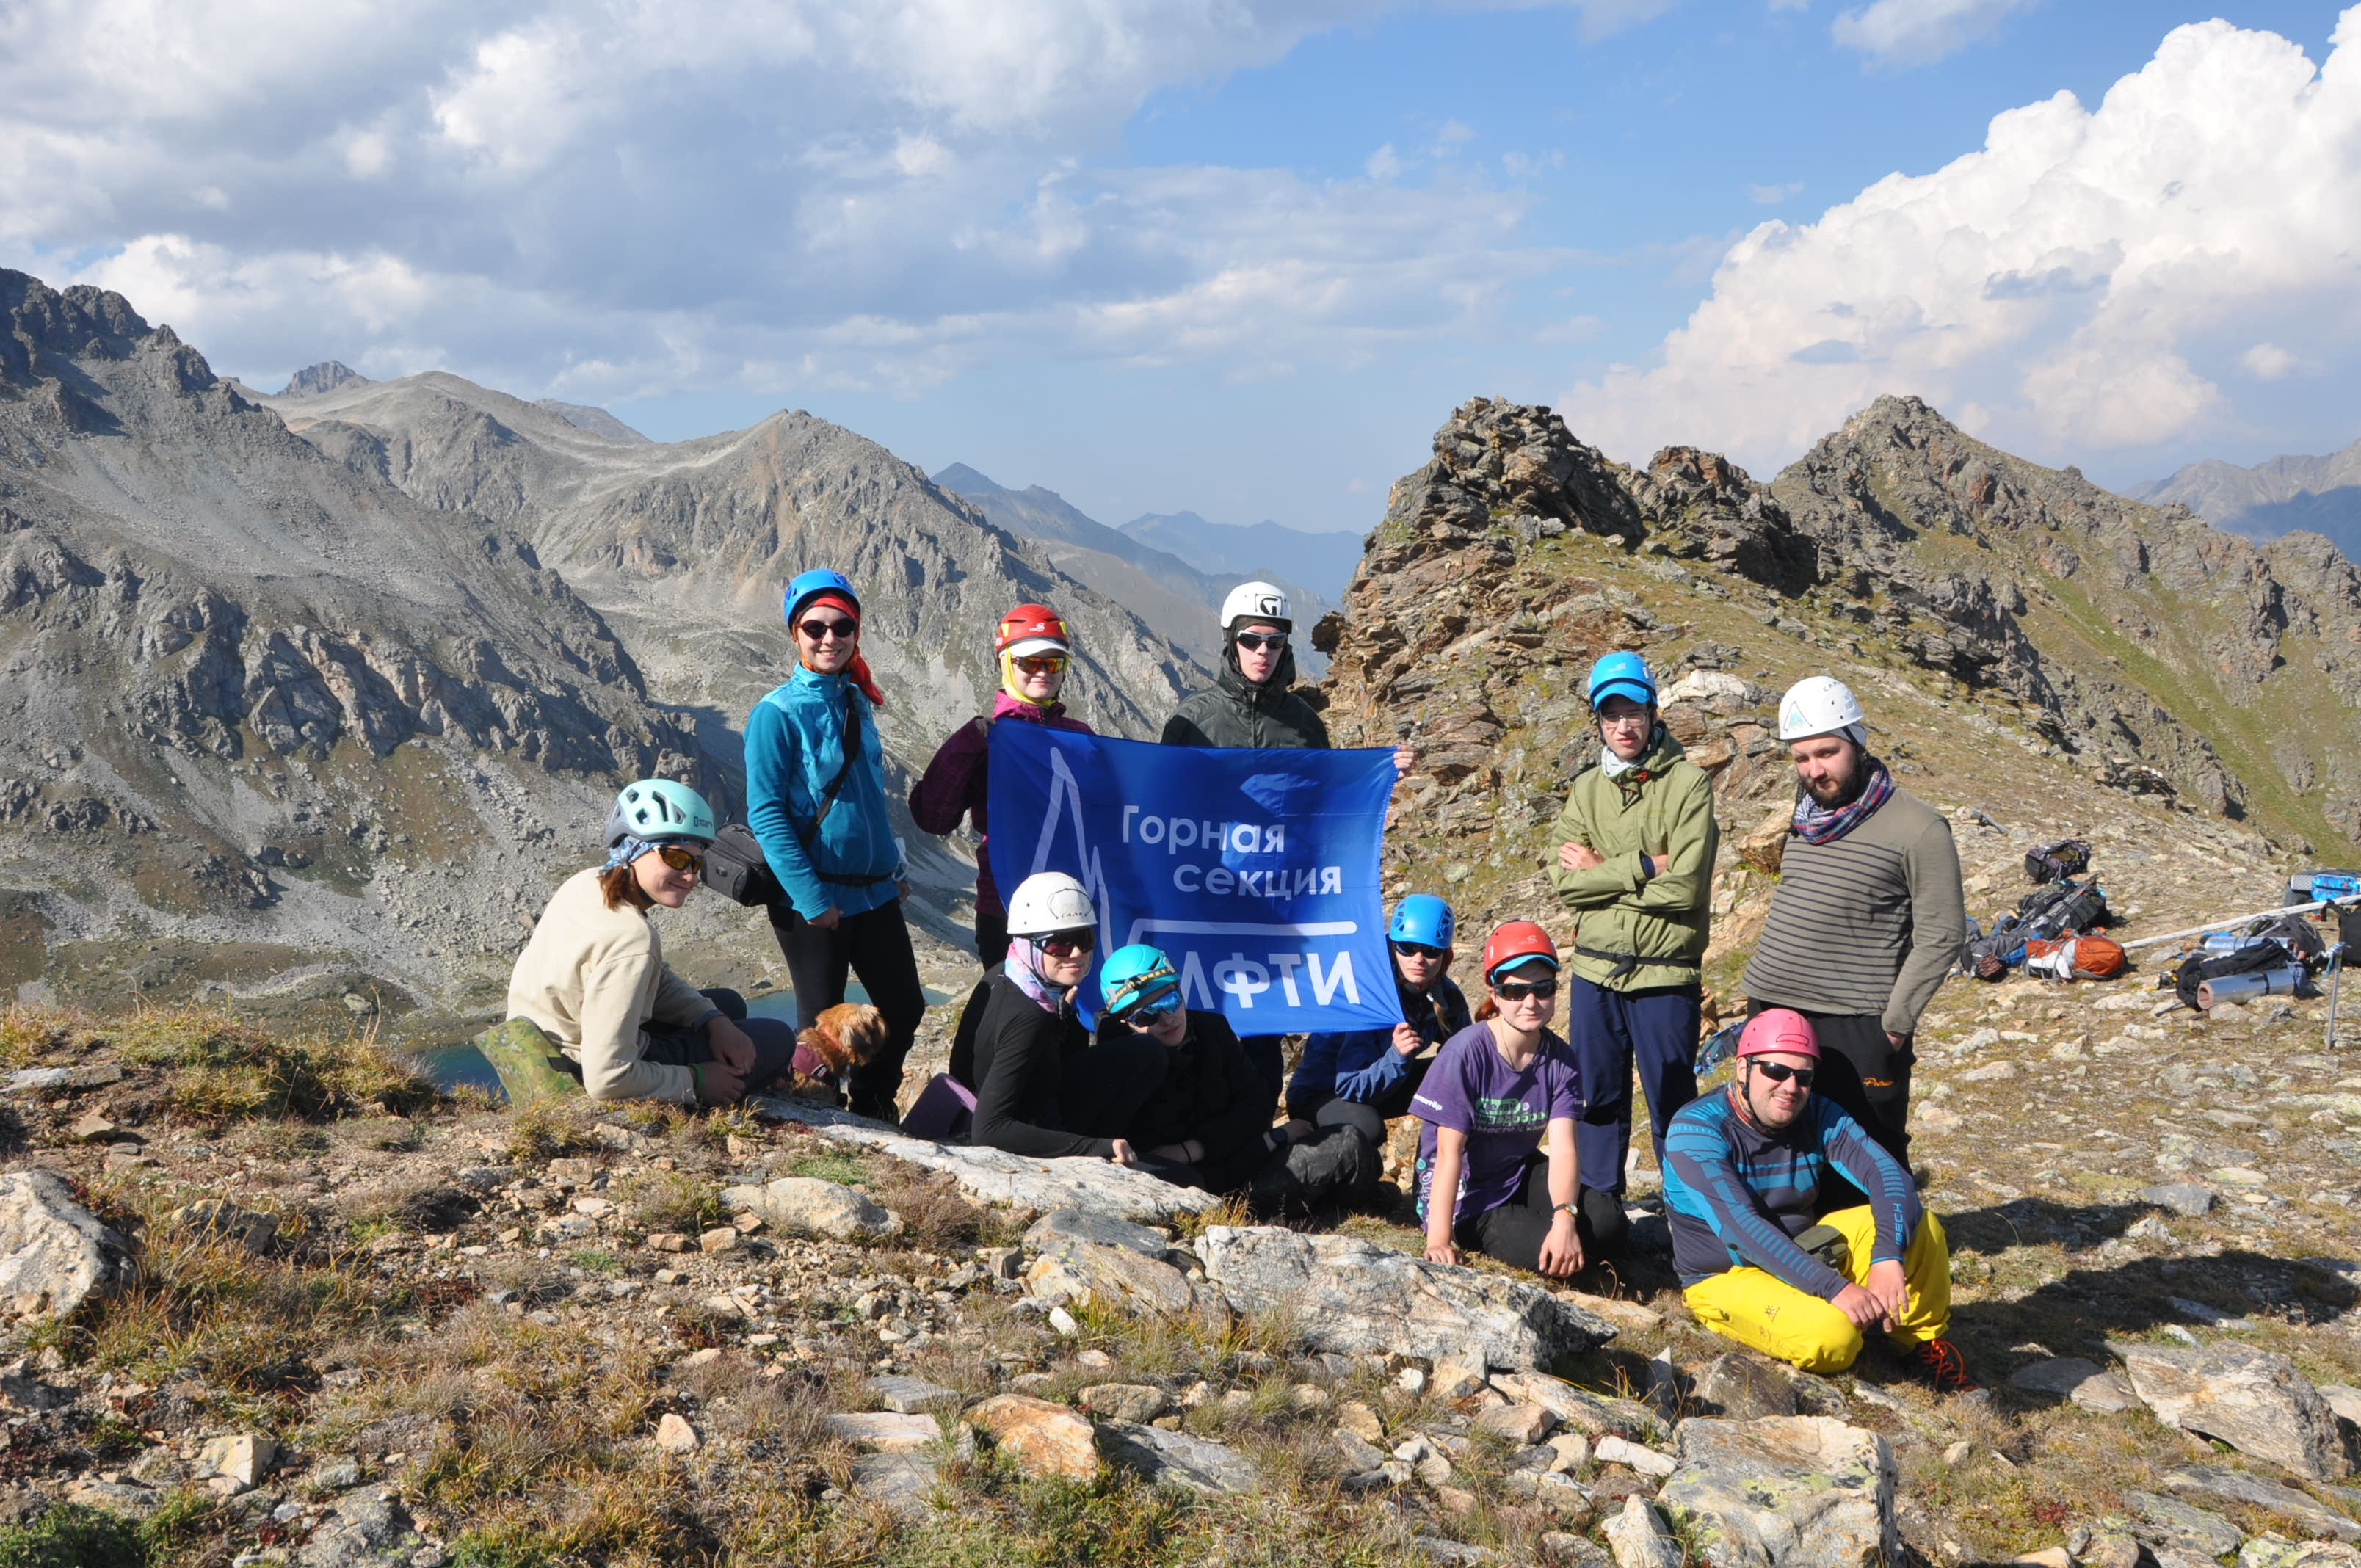
\includegraphics[width=0.7\linewidth]{../pics/DSC_0986}
	\caption{Группа на перевале, вид на оз. Уллу-Кёль}
	\label{fig:DSC_0986}
\end{figure}


В 15:48 выходим на спуск. Катя чувствует себя хорошо и идёт со своим рюкзаком.
Спускаемся к озеру по пологому травянистому склону, далее--- по гребню.

\begin{figure}[h!]
	\centering
	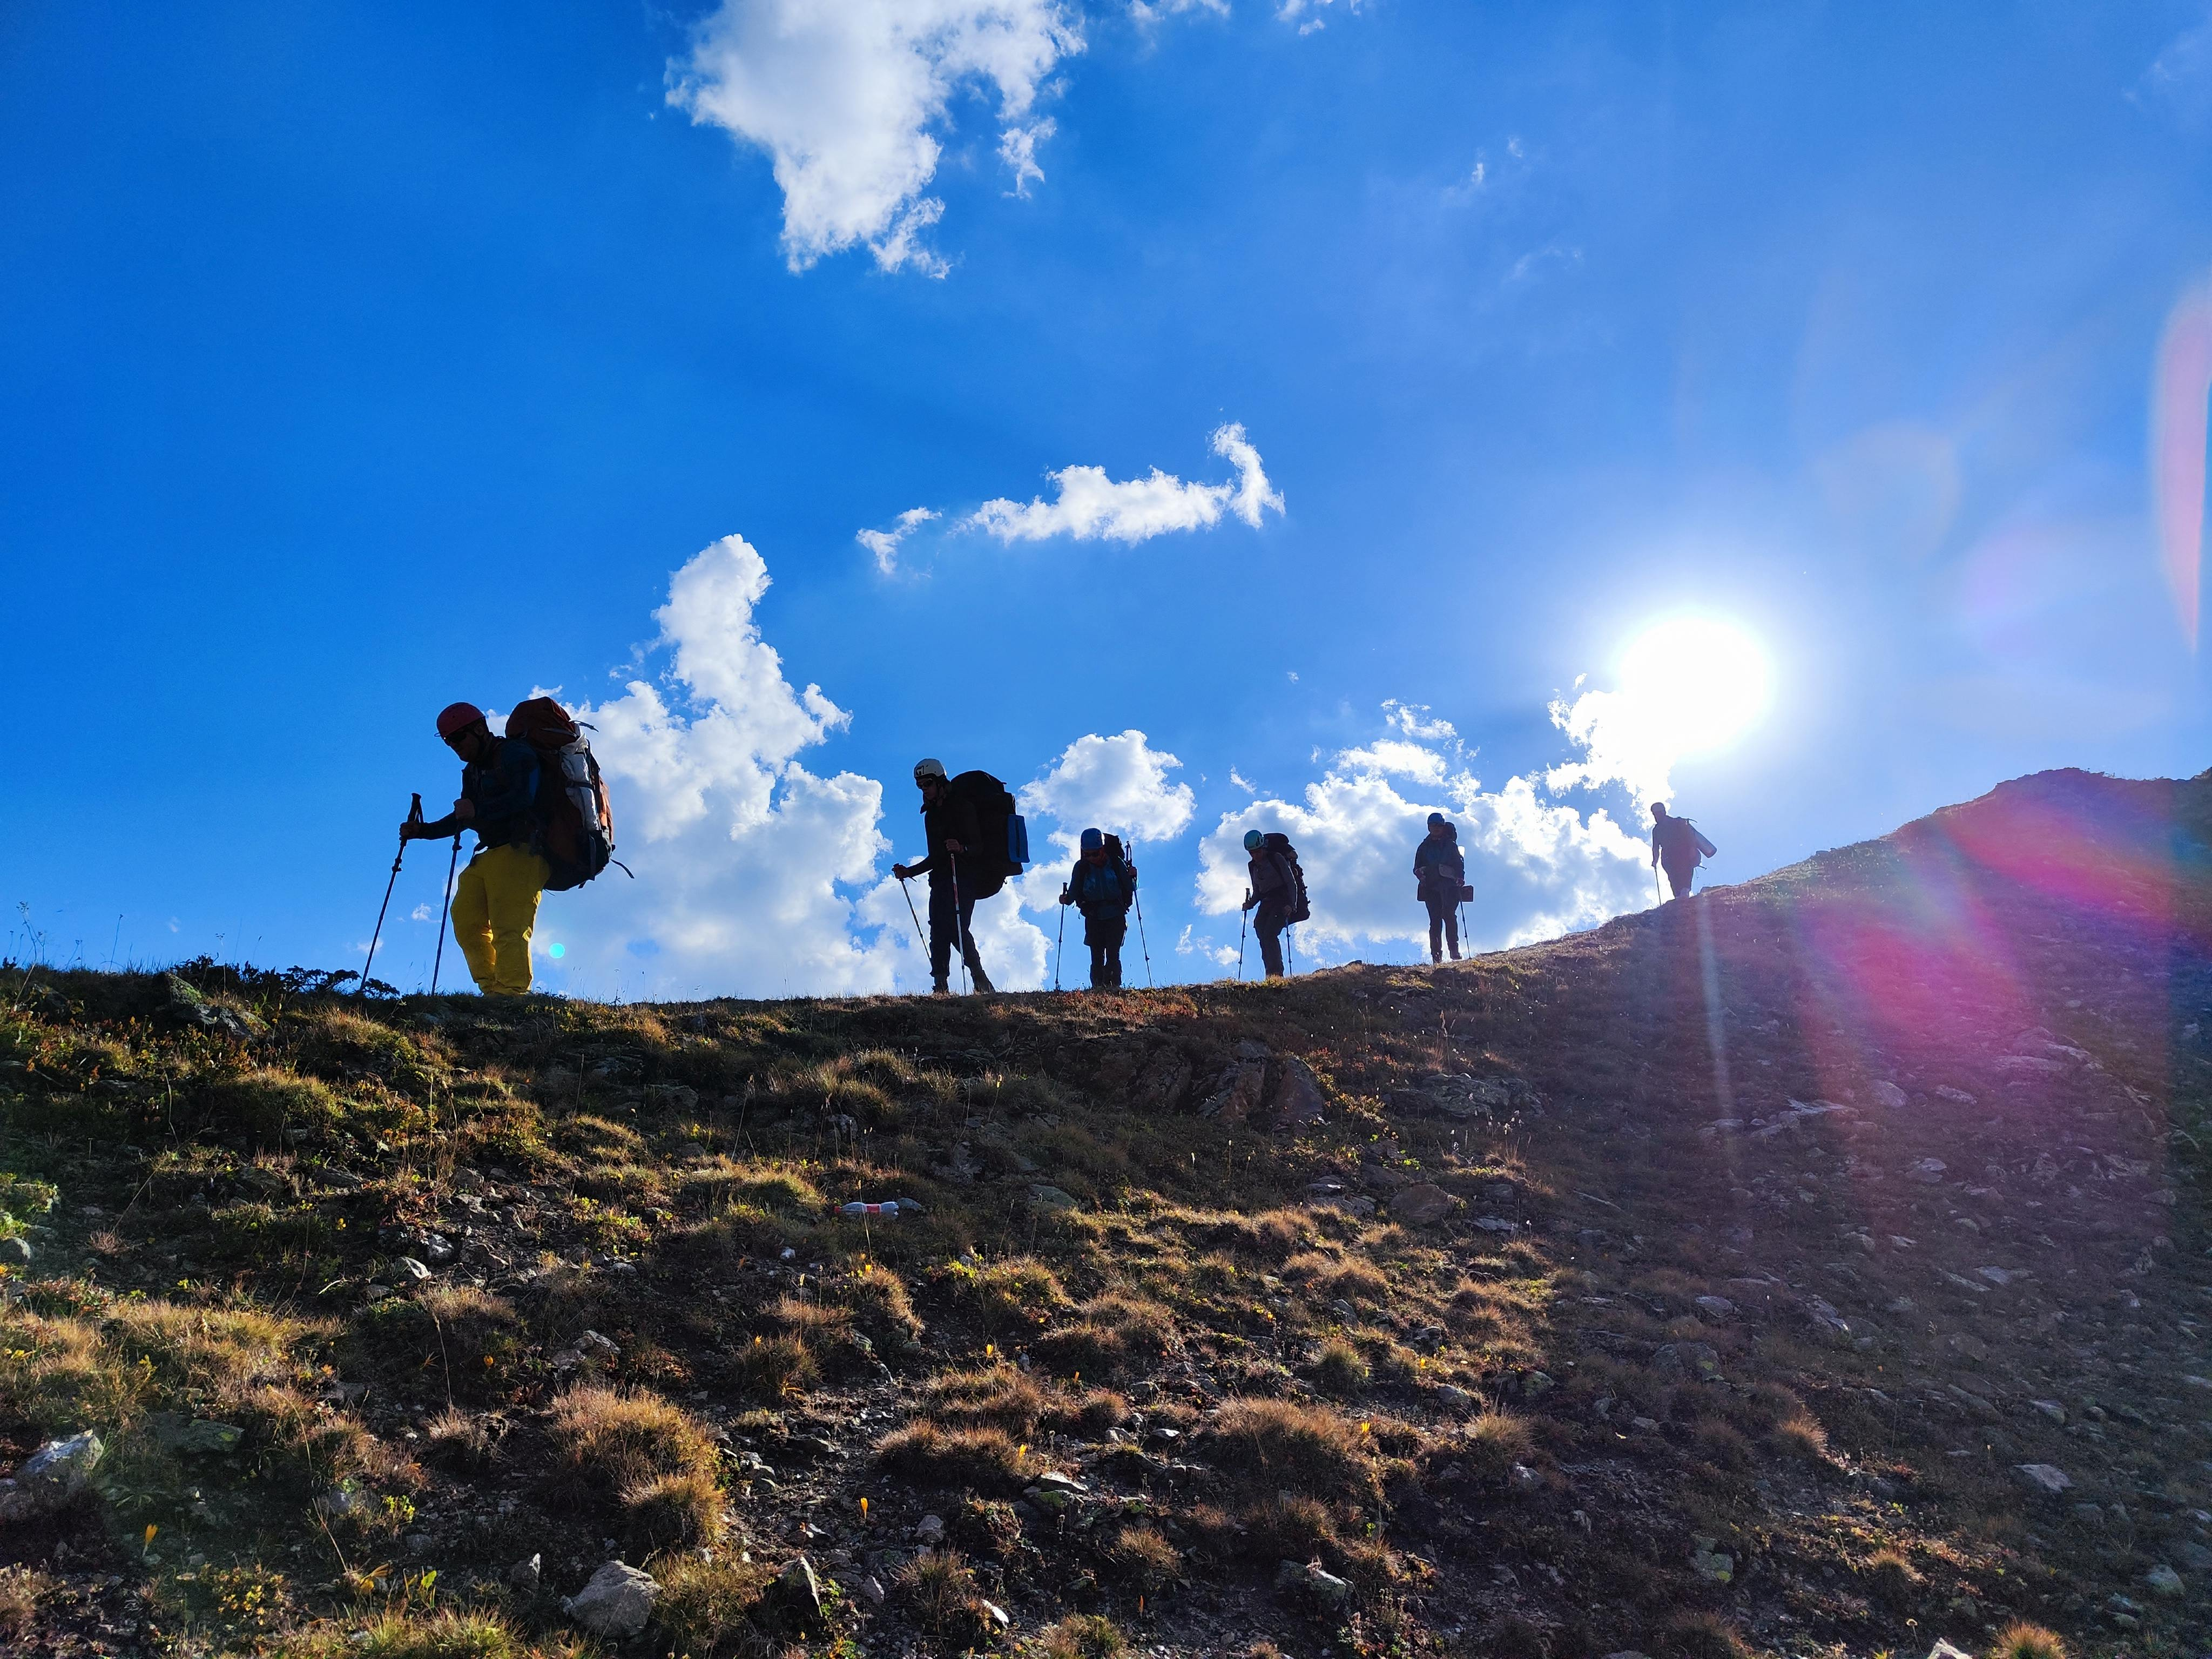
\includegraphics[width=0.7\linewidth]{../pics/IMG_20240820_164917.jpg}
	\caption{Спускаемся по гребню к озеру}
	\label{fig:IMG_20240820_164917.jpg}
\end{figure}

Приходим на озеро в 16:52, устраиваем обед. В 18:10 выходим, по дороге думаем. стоит ли ночевать у коша пастухов или лучше спуститься в д.р. Махар (рис.~\ref{fig:20240820_184645.jpg}).

\begin{figure}[h!]
	\centering
	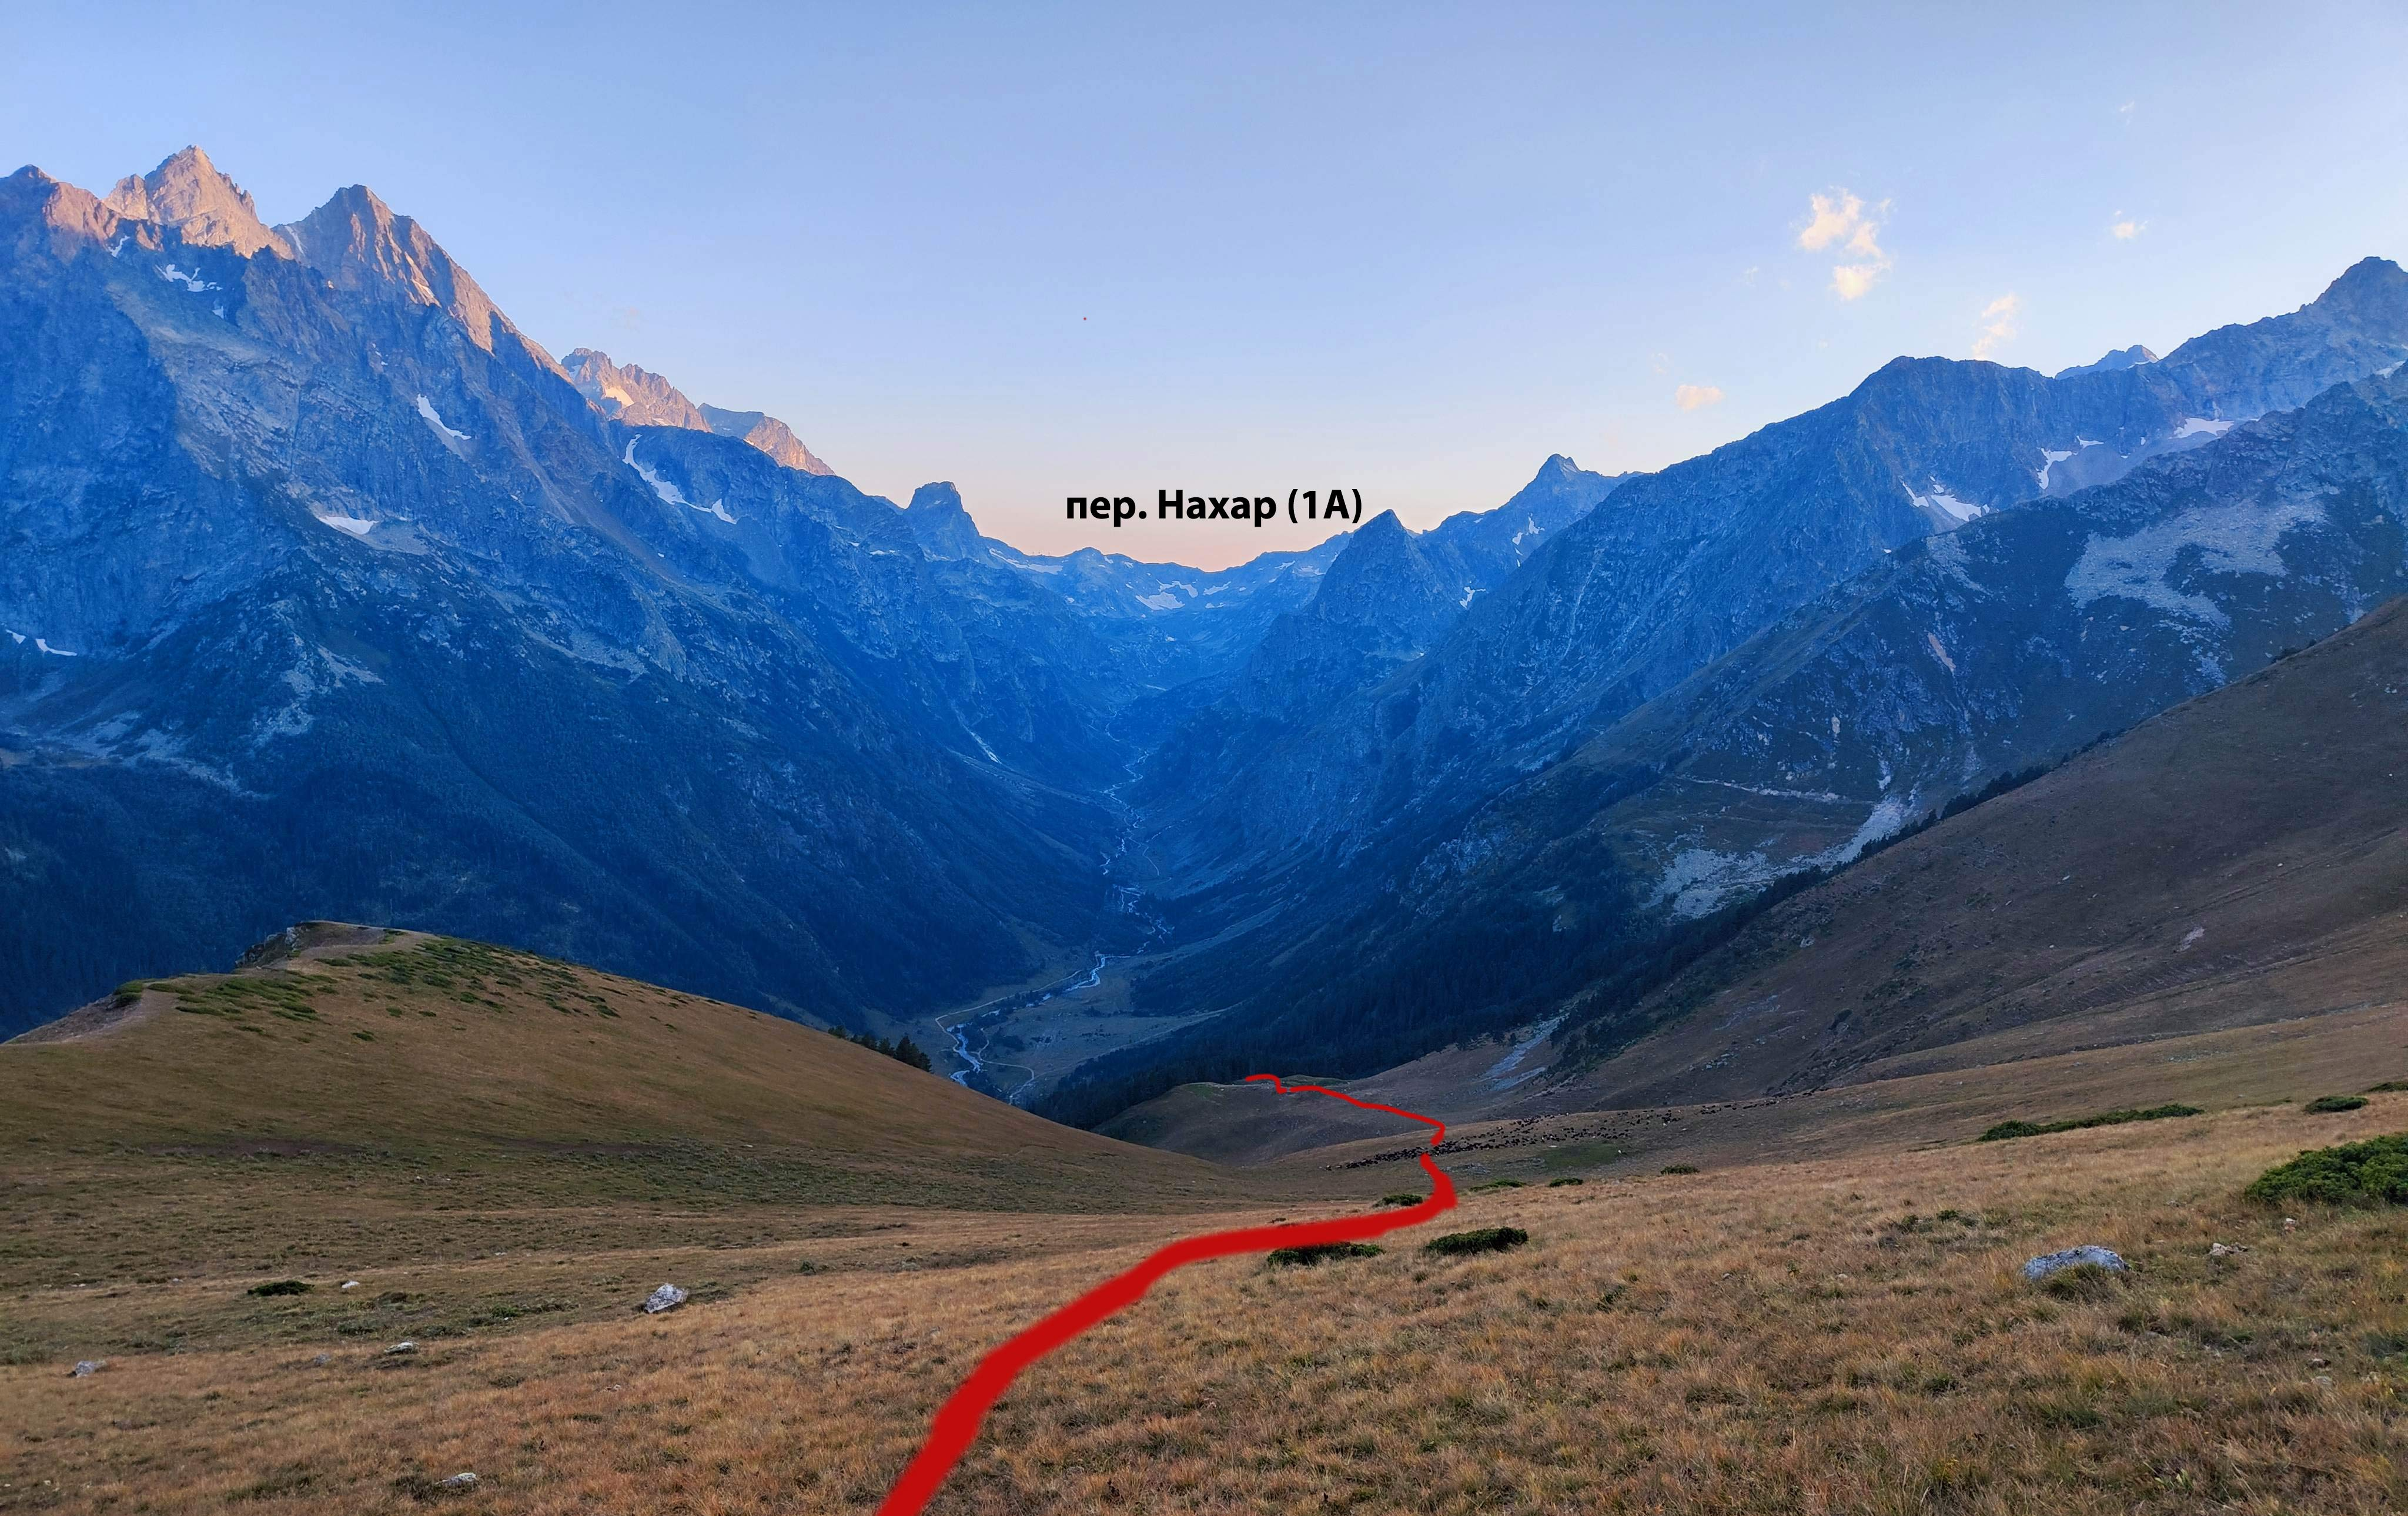
\includegraphics[width=0.7\linewidth]{../pics/IMG_20240820_184645.jpg}
	\caption{Спуск в д.р. Махар}
	\label{fig:IMG_20240820_184645.jpg}
\end{figure}

Спускаемся к кошу в 20:16. Уже темно, идём с фонариками. Узнаём у пастуха, что до долины 1.5~км по хорошей тропе, что вкупе с небольшим сбросом (300 м) сподвигает участников проголосовать за спуск в долину и ночёвку внизу. Спуск технически несложный, мешали спуску разве что пыль и мошки. Также сказывается общая усталость группы. На начальном участке тропа узкая, в момент выхода к р. Трёхозёрнаяя становится шире.

В 22:15 встали на ночёвку в д.р. Махар, координаты м.н. N43.294527\degree,~E41.956866\degree.


\clearpage
